%%%%%%%%%%%%%%%%%%%%%%%%%%%%%%%%%%%%%%%%%
% Lachaise Assignment
% LaTeX Template
% Version 1.0 (26/6/2018)
%
% This template originates from:
% http://www.LaTeXTemplates.com
%
% Authors:
% Marion Lachaise & François Févotte
% Vel (vel@LaTeXTemplates.com)
%
% License:
% CC BY-NC-SA 3.0 (http://creativecommons.org/licenses/by-nc-sa/3.0/)
% 
%%%%%%%%%%%%%%%%%%%%%%%%%%%%%%%%%%%%%%%%%

%----------------------------------------------------------------------------------------
%	PACKAGES AND OTHER DOCUMENT CONFIGURATIONS
%----------------------------------------------------------------------------------------

\documentclass{article}

\input{structure.tex} % Include the file specifying the document structure and custom commands

%----------------------------------------------------------------------------------------
%	INFORMATION
%----------------------------------------------------------------------------------------

\title{Open Source Roboter Plattform} % Title

\author{Lukas Reichwein\\ Yves Ehrlich\\ Nick Gnoevoj}

\date{University of Applied Science Fulda --- \today} % University, school and/or department name(s) and a date

%----------------------------------------------------------------------------------------

\begin{document}

\maketitle % Print the title
\tableofcontents % Inhaltsverzeichniss, Achtung zweimal Compilerien!
\newpage

%----------------------------------------------------------------------------------------
%	INTRODUCTION
%----------------------------------------------------------------------------------------

\section{Vorwort} % Unnumbered section
    \paragraph{Motivation}
    Eine Plattform bieten ist etwas, das momentan sehr stark im Trend liegt, sei es im Software oder im Hardware Bereich. Im Softwarebereich zeigt sich dies meist durch Open-Source Bibliotheken, welche möglichst variabel einsetzbaren Code für jeden frei zugänglich machen. \\    
    Ein solches Projekt war auch von einem der Projektmitglieder (Yves Ehrlich) als Privates Projekt geplant und so kam die Überlegung dies innerhalb des Modules Embedded Networking zu wählen.\linebreak
    \paragraph{Basis des Projektes}
    Als Basis des Projektes dient einer schon bereits von Yves Ehrlich angefertigter Arduino Nano Shield samt Code,
    \cite{nanoGame} welcher als Fernsteuerung verwendet wird. 
    \paragraph{Ziel des Projektes}	
	Ziel des Projektes ist ein ferngesteuerte, Open-Source basierende Roboterplattform.

\newpage    
\section{Überlegung}%Yves

Die urprüngliche Idee war die Entwicklung eines Solarroboters, also eines Roboters, der tagsüber mit Hilfe der Sonneneinstrahlung seinen Eigenbedarf decken kann und somit nur einen kleinen Pufferakku benötigt.
Praktische Anwendungen könnten z.B. die Nutzung als kompakte Straßenkehrmaschine oder als Rasenmäher sein. Bedingt durch die eingeschränkte Leistungsabgabe der Solarzellen vermutlich nur für kleine zu bearbeitende Flächen.
Da es nur wenige brauchbare und frei zugängliche Quellen für solche Plattformen gibt, wollten wir eine eigene schaffen. Daher sollte das Projekt exemplarisch als Grundlage für eine Quelloffene Plattform dienen, die auch von anderen genutzt und weiterentwickelt werden kann.

Da wir bei der Entwicklung der mechanischen Komponenten schnell feststellen mussten, dass das Fahrwerk recht komplex ist, insbesondere die Vorderachse, schwenkten wir schnell auf eine andere Bauweise um. Zunächst war der Aufbau mit 4 gleichen Rädern geplant, von denen zwei Stück (Hinterachse) von einem bürstenlosen Gleichstrommotor angetrieben werden sollten. Die Entwicklung eines Differenzials gestaltete sich noch als relativ einfach. Die Vorderachse aber mit dem Servo gestaltete sich dann, hinsichtlich des Zeitaufwandes, für zu komplex.

\begin{figure}[h]
	\includegraphics[width=12cm]{hinterachse.png}
	\centering
	\caption{Hinterachse des urpsrünglichen Aufbaus}
\end{figure}

\begin{figure}[h]
	\includegraphics[width=12cm]{lagerschalen.png}
	\centering
	\caption{Lagerschalen}
\end{figure}

Somit schwenkten wir kurzer Hand zu einem sehr viel einfacheren Aufbau um, um uns schneller den wichtigeren Komponenten widmen zu können.
Der neue Aufbau sah eine schlichte Grundplatte als Plattform für die weiteren Bauteile, wie Motoren (Mabuchi N20 mit Getriebe), Ultraschallsensor, Akku, Hauptplatine und uvm. vor.
Um möglichst viele Montagemöglichkeiten zu bieten, wurde die Grundplatte mit Bohrungen in regelmäßigen Abständen versehen. Diese Bohrungen können zum durchstecken für Schrauben oder zum versenken von Gewindemuffen genutzt werden.
Zum anbringen unserer Komponenten haben wir auf Messinggewindebuchsen und passende M3 Schrauben gesetzt.
Alle selbstentworfenen Komponenten haben wir mit einem FFF 3D-Drucker aus PLA gedruckt.
Mit Ausnahme der Hauptplatine natürlich.
Bedingt durch den Zeitaufwand des gesamten Projektes und anderer Studienmodule haben wir uns entschieden, die Implementierung eines MPPT Ladereglers fallen zu lassen, somit wurde die Idee des Solarroboters auf die Idee der Entwicklung eines Roboters reduziert.

\newpage

\begin{figure}[h]
	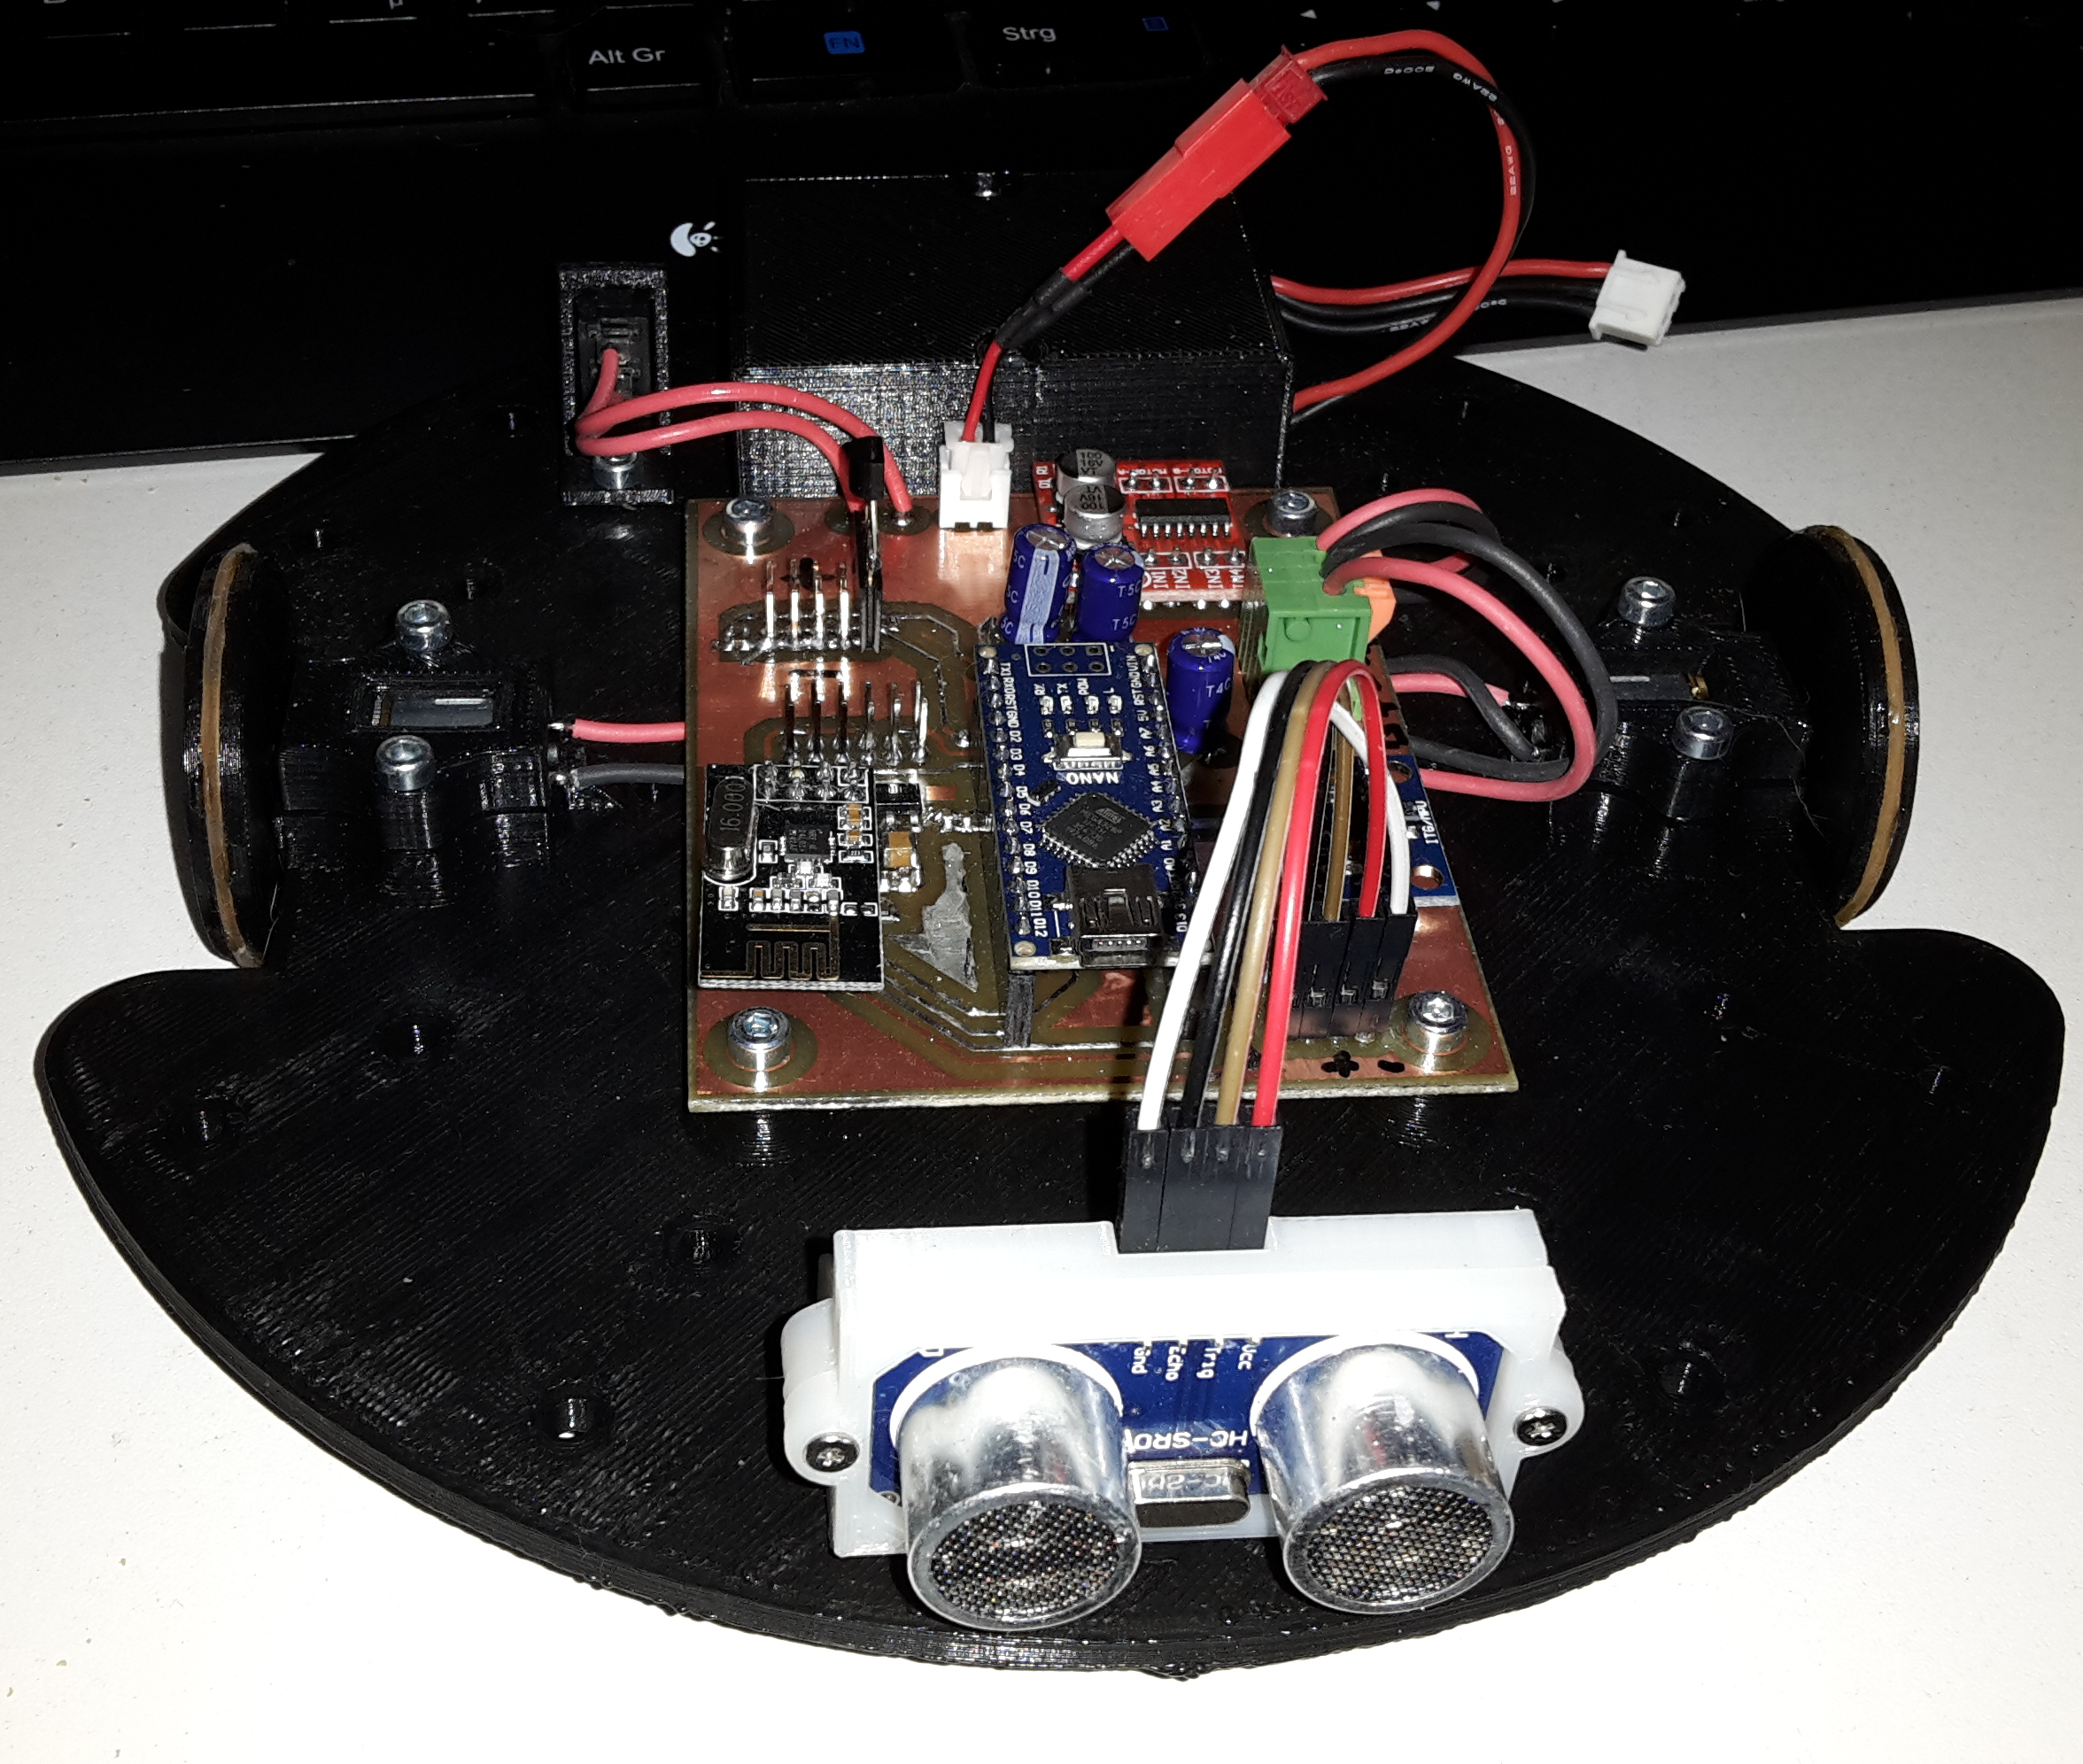
\includegraphics[width=12cm]{roboter.png}
	\centering
	\caption{Der Roboter, aktueller Aufbau}
\end{figure}

\newpage    
\section{Mechanik}%Yves

Wie bereits unter „Überlegung“ erwähnt, gestaltete sich der Aufbau mit Achsträger, Radlager und Lagerschalen uvm. als zu Zeitintensiv um in der vorgegebenen Zeit bewältig werden zu können.
Zum Entwurf der mechanischen Bauteile wurde das CAD Programm Fusion 360 von Autodesk verwendet. Dabei gab es kaum Schwierigkeiten, da Yves bereits sehr viel Erfahrung mit 3D-CAD Programmen gesammelt hat. Lediglich der Zwang Windows zu benutzen stellt eine ständige Unannehmlichkeit dar.

Alle Entwürfe wurden mit einem 3D Drucker gedruckt, einem HCmaker7, ein Klon des bekannten Creality CR-10S.
Das Material der Wahl war PLA. Für einen Außeneinsatz ist das Material wegen der geringen Witterungsbeständigkeit kaum geeignet. Insbesondere die geringe Temperaturbeständigkeit (max. 60°C) disqualifizieren das Material für den Einsatz in der Sonne. Da dies aber ohnehin nicht mehr geplant war, ist das Material für unseren Zweck geeignet.

Die Gewindebuchsen in den Kunststoff einzusetzen ist relativ einfach, man benötigt dafür lediglich eine Schraube die man in die Buchse einschraubt und einen Lötkolben mit einer Temperatur von etwa 240°C. Ohne Druck auszuüben legt man die Spitze des Lötkolbens auf den Schraubenkopf. Wenn die Schraube ausreichend Wärme an die Muffe übertragen hat, fängt die Muffe an im Kunststoff zu versinken. Die Schwerkraft sorgt hier für alles nötige. Wenn die Muffe weit genug versunken ist, kann der Lötkolben entfernt werden und man sollte die Schraube schnell abkühlen, z.B. durch pusten oder ein kleines Gebläse wie z.B. einen Radiallüfter.
Beim Design der Kunststoffteile muss man darauf achten, dass für Gewindemuffen stehts eine ausreichend große Fase vorhanden sein muss, damit die Muffe einerseits zentriert wird beim versinken und andererseits kein verdrängtes Material die Muffe beim versinken behindert oder verstopft. Letzterem wird aber auch durch die eingeschraubte Schraube vorgebeugt.

Da Kunststoffe auf glatten Oberflächen sehr wenig Bodenhaftung haben, wurden die Räder mit einer Nut versehen. In diese Nut kann man später ein einfaches Haushaltsgummiband einlegen, somit hat der Roboter auch auf glatten Oberflächen relativ gute Haftung.

Der Aufbau sieht zwei Antriebsmotoren vor, welche jeweils ein Rad treiben. Zum abstützen verfügt der Roboter über ein selbstentworfenes Kugelrad. Dieses Kugelrad verwendet als Kugeln vier handelsübliche Airsoft Kugeln mit einem Durchmesser von 6mm.
Die Gleiteigenschaften dieser Konstruktion sind nicht die besten, aber für diesen Prototypen ausreichend. Um die Reibung zu vermindern haben wir Silikonöl auf die Kugeln aufgetragen.

\newpage    
\section{Elektronik}%Yves

Lochrasterplatinen, wie sie häufig für Prototypzwecke genutzt werden, sind nicht nur unpraktisch für SMD Komponenten, auch wenn man ein 2,54mm Raster mit einigen Tricksereien durchaus auch für SMD Komponenten nutzen kann, sie sind auch relativ unzuverlässig und die Fehlersuche gestaltet sich z.T. als schwierig (je nach Menge und Komplexität der Verdrahtungslagen).
Deshalb entschieden wir uns, eine eigene Platine zu entwickeln.
Als Software nutzten wir dafür das kommerzielle Programm Sprint Layout 6 von der Firma Abacom.

Da die Herstellung der Platine von Hand erfolgen sollte, haben wir die Strukturen der Platine sehr grob gezeichnet. Was auch durch die geringe Anzahl an Komponenten und deren modulare Bauweise begünstigt wurde.

\section{Verfahren}%Yves

Als Verfahren zum beschichten der Platine diente die Tonertransfermethode. Dabei wird die Schaltung mit einem Laserdrucker auf geeignetes Papier gedruckt, in diesem Fall Photopapier, und dann mit Hitze auf die blanke Platine gedrückt. Für diesen Zweck hat Yves ein Laminiergerät umgebaut, welches den Vorgang erheblich erleichtert.
Da unsere Platine doppelseitig ist, müssen zuvor die zwei Seiten, welche die Schaltung enthalten Deckungsgleich aufeinander ausgerichtet werden und dann an den Rändern verklebt werden, damit man am Ende eine Art Tasche erhält, in welche dann die Platine eingesteckt werden kann.
Das ganze läuft dann einige Male durch das Laminiergerät. Nach dem das erfolgt ist, lässt man die Platine etwas abkühlen und ab einer Temperatur von etwa 30-40°C schneidet man die Tasche seitlich auf und zieht vorsichtig das Papier ab. Der Toner bleibt am Kupfer haften und schützt an diesen Stellen, wie ein Fotolack, das Kupfer davor weggeätzt zu werden.
Anschließen gibt man die beschichtete Platine in eine Ätzküvette welche mit einer Natriumpersulfat-Lösung gefüllt ist. Nach einiger Zeit kann man beim durchleuchten der Küvette sehen, wie sich das Kupfer immer weiter auflöst, bis am Ende die Schaltung klar und deutlich zu sehen ist. Dann wird die Platine entnommen und gründlich mit Wasser abgespült.
Zum entfernen des Toners benötigt man etwas Aceton und einen Lappen.
Für die THT Komponenten müssen nun noch Bohrungen gesetzt werden. 1,2mm, passend für die Durchkontaktiernieten von Bungard.
Nach dem verpressen (mangels passender Presse eher mit einem Körner breitschlagen) der Nieten, müssen diese beidseitig verlötet werden. Danach können alle Komponenten bestückt werden.

\begin{figure}[h]
	\includegraphics[width=16cm]{laminiergeraet.png}
	\centering
	\caption{Laminiergerät}
\end{figure}

%Platine 
\begin{figure}[h] 
    \subfigure[Top-Layer]{\includegraphics[width=8cm]{pcbTop.png}} 
    \subfigure[Bottom-Layer]{\includegraphics[width=8cm]{pcbBottom.png}} 
\caption{fertig geätzte Platine} 
\end{figure} 

\newpage
\section{Bestücken}%Yves

Zum verlöten der Komponenten kam Feinlot mit Bleianteil zum Einsatz.
Für SMD Komponenten wurde eine Pinzette als Hilfswerkzeug verwendet.

\section{Schaltung}%Yves

Die Schaltung ist relativ einfach gehalten. Im wesentlichen dient die Platine nur als Träger für die modularen Komponenten und für diverse Anschlussmöglichkeiten. Für den NRF24 wurde ein 3,3V Spannungsregler integriert.
Um etwaige Motorenwechsel zu erleichtern, sind zu deren Anschluss Federzugklemmen verbaut worden.
Wegen der Überschaubarkeit der Schaltung haben wir auf einen Schaltplan verzichtet, da das Layout selbsterklärend ist.

\section{Fernsteuerung}%Yves

Auf die Fernsteuerung soll an dieser Stelle nicht näher eingegangen werden, da diese zum Zeitpunkt der Erstellung dieses Projektes bereits „fertig“ war.
Es wurden lediglich ein Joystick sowie ein NRF24 ergänzt.
Detaillierte Informationen finden sich im dazugehörigen Repositorium.

Im Rahmen eines Arduino Workshops für Anfänger entwickelte Yves eine Platine, welche als Shield für einen Arduino Nano fungiert. Sie enthält grundlegende Dinge wie Tasten, einen Akku, eine stabile 5V Spannungsversorgung sowie ein monochromes LCD Display mit Hintergrundbeleuchtung, um nur die wichtigsten Sachen zu nennen.

Dank der Buchsenleiste auf der Rückseite, welche neben 3,3V und 5V Spannungsversorgung auch diverse I/Os und Analogeingänge bereitstellt, lässt sich das Shield „nanoGame“ hervorragend erweitern und für viele verschiedene Dinge nutzen, so auch als Fernsteuerung für unseren Roboter.

Bei dem Joystick handelt es sich um eine Platine welche ein original Ersatzteil der Sony PSP enthält. Dieser Joystick ist sehr kompakt und ließ sich dadurch recht einfach in unsere Projekt integrieren. Es musste lediglich eine Halterung konstruiert werden, um den Joystick an das Gehäuse der Fernsteuerung zu schrauben.

Beim Funkmodul sind wir kompromissloser vorgegangen. Dieses wurde mit ein wenig Silikonklebstoff an der Oberseite fixiert.

Alle Verbindungsleitungen wurden Freiluft auf der Rückseite der Fernsteuerung zum Schacht der bereits erwähnten Buchsenleiste gelegt und dort mit Steckerleisten angeschlossen.

\begin{figure}[h]
	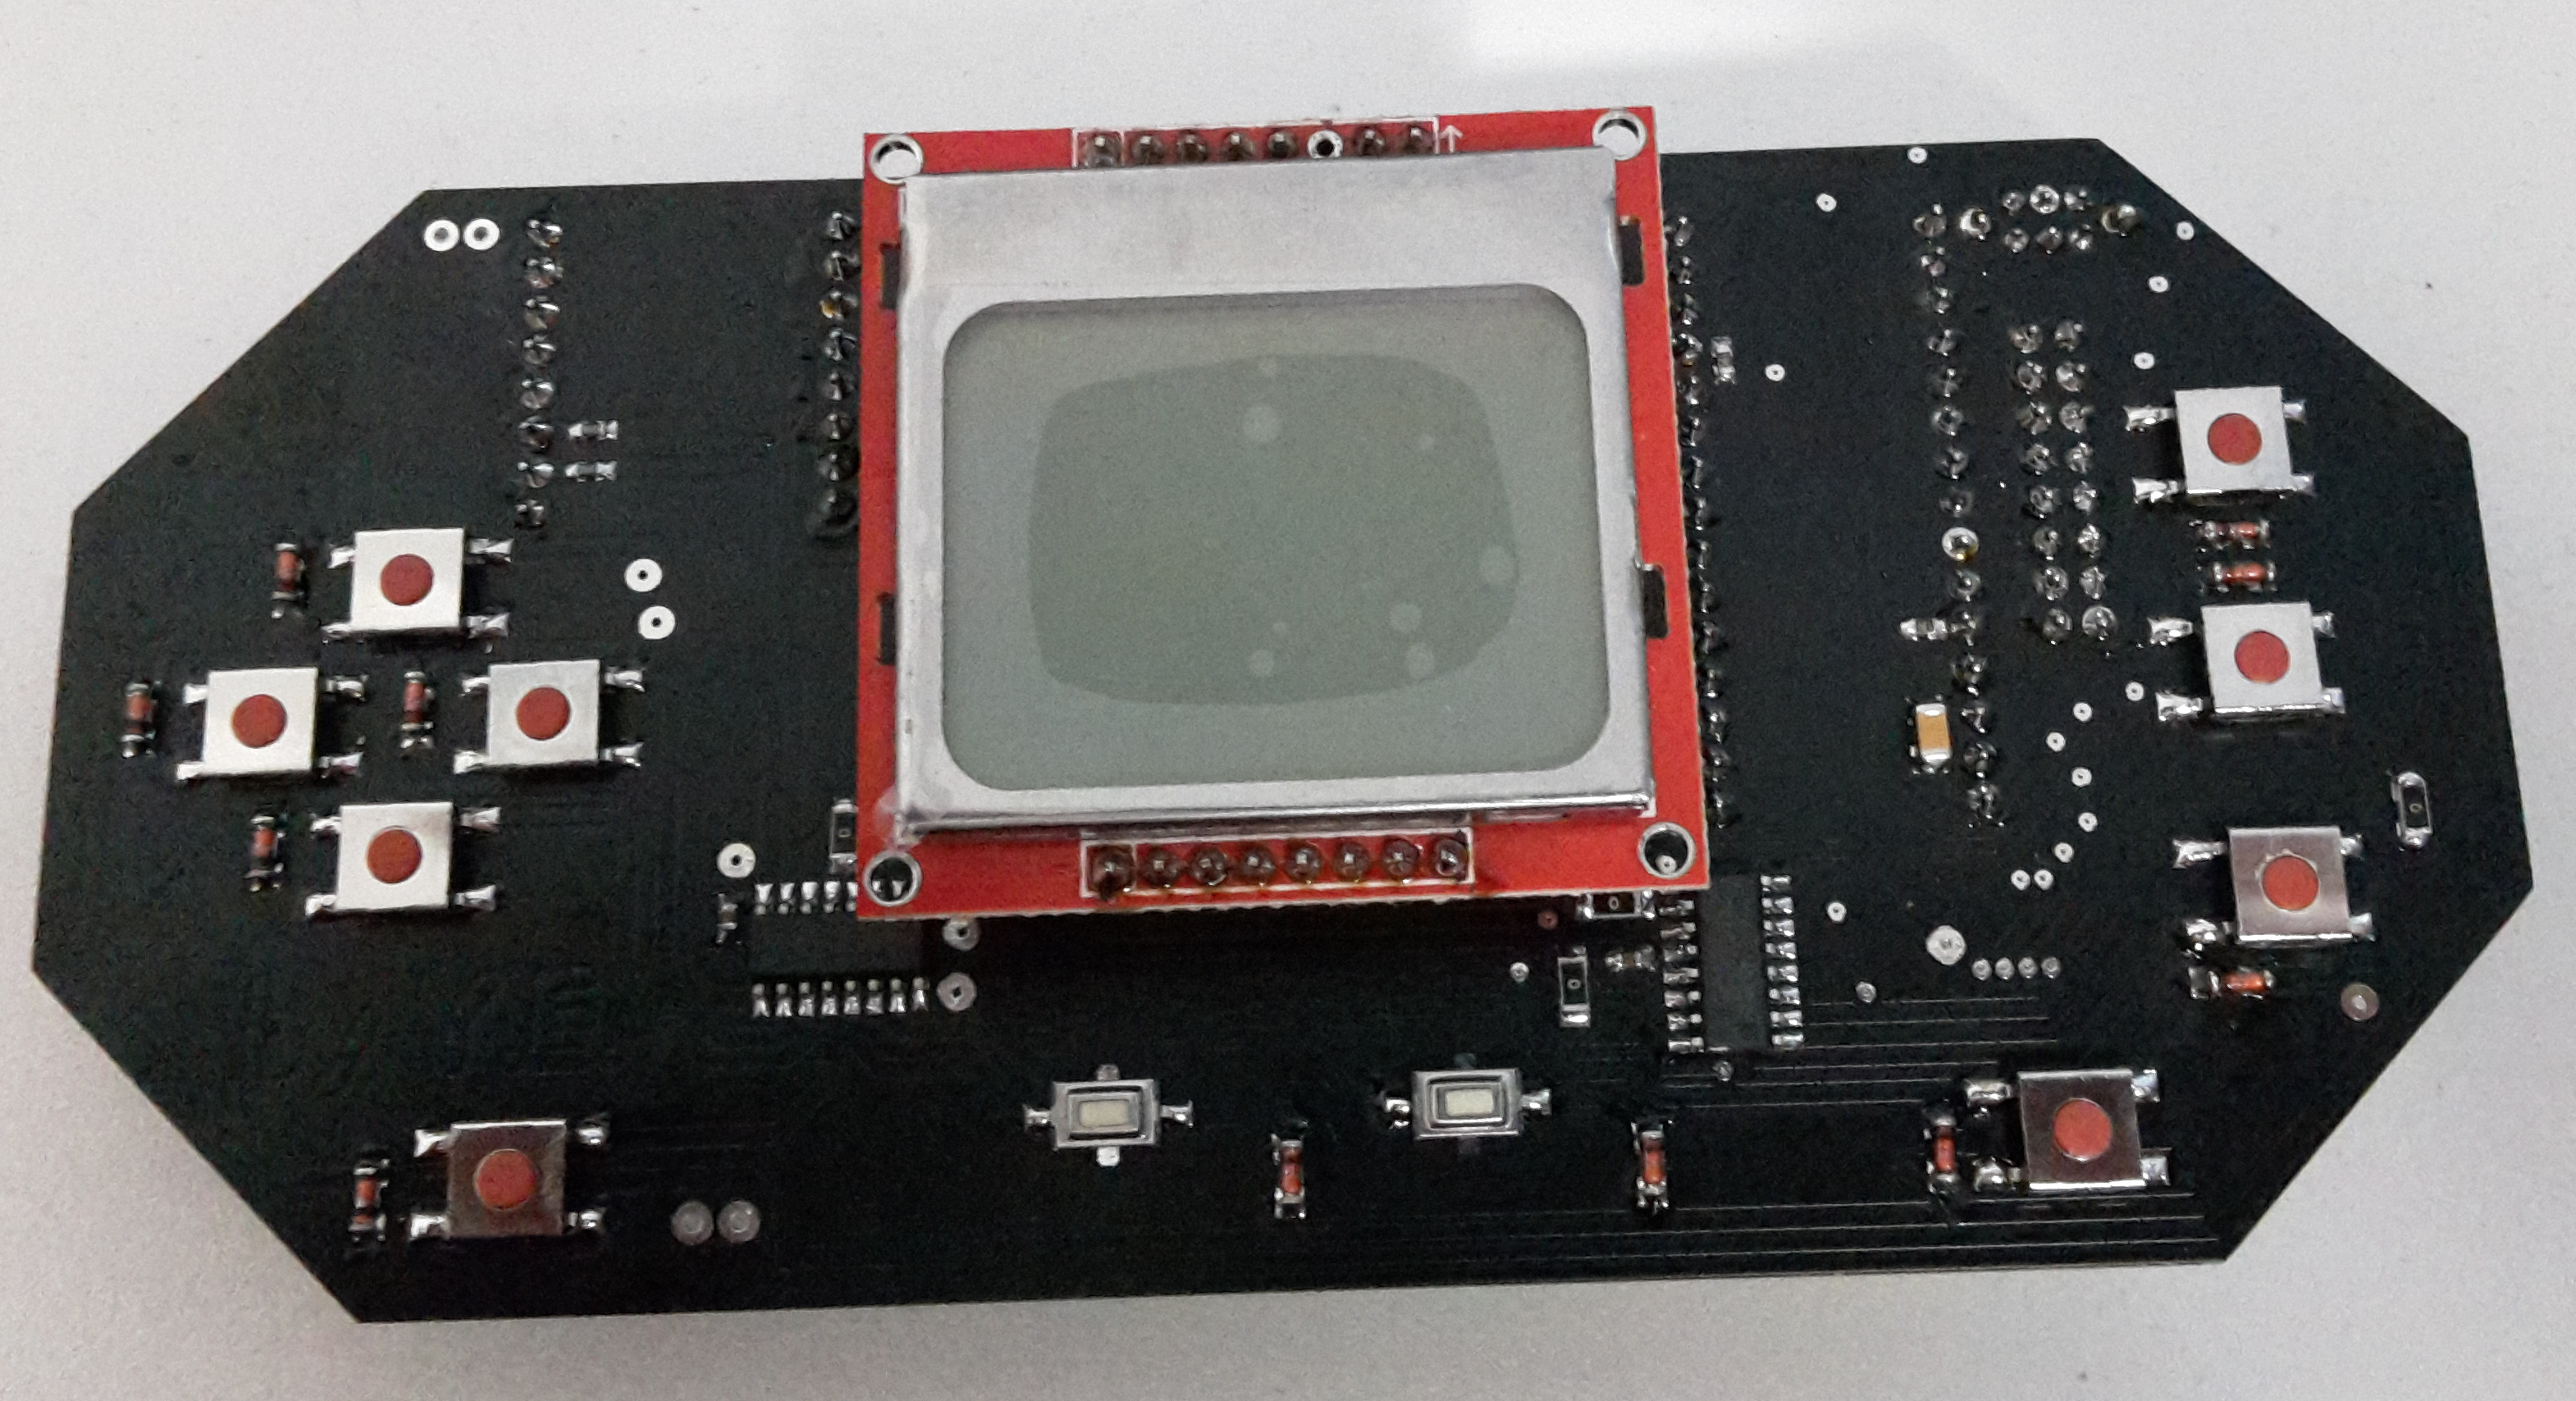
\includegraphics[width=12cm]{rcVorn.png}
	\centering
	\caption{Fernsteuerung vorn}
\end{figure}

\begin{figure}[h]
	\includegraphics[width=12cm]{rcHinten.png}
	\centering
	\caption{Fernsteuerung hinten}
\end{figure}

\newpage
\section{Code allgemein}%Yves

Um die Einsatzmöglichkeiten für den Code möglichst flexibel zu gestalten, haben wir uns bemüht, nicht blockierenden Quelltext zu schreiben.
Somit lässt sich auch mit dem recht kleinen Atmega328p bei 16 MHz Takt eine ganze Menge bewältigen.

Aktuell ist der Roboter in der Lage auf Kommandos, die er von der Fernsteuerung erhält, zu reagieren. Aus Zeitgründen konnten wir leider nur einen manuellen Fahrmodus implementieren. Dieser beinhaltet das fahren mit digitalen Tasten sowie „analog“ mit dem ergänzten Joystick.
Weiterhin implementiert wurden das erfassen von Temperaturen mit Hilfe eines DS1820 und eine Distanzmessung mit einem HC-SR04 Ultraschallsensor.

Die Übertragung von Kommandos ist relativ einfach gehalten. Das erste Byte im commands Array ist ein Kommando, gefolgt von 2 Bytes mit Daten. Diesem Muster folgend ist jedes dritte Byte ein Kommando, gefolgt von zwei Datenbytes.
Da das Array eine feste Größe von 32 Byte hat, lassen sich folglich bis zu 10 Kommandos übertragen. Wie viele Kommandos jeweils übertragen werden und in welcher Reihenfolge diese im Array vorkommen, also ob Byte 0,3,6,9...usw., spielt keine Rolle.

\newpage    
\section{SPI}%Lukas

\newpage
\section{Funksteuereung} %Lukas
    Wie schon zuvor erwähnt wird für die Basis der Funksteuerung das Arduino Shield verwendet, welches mit einem RF24 Chip erweitert wurde.
    \subsection{RF24} %Oder nur als paragraph je nachdem wie viel zusammen kommt.
       Die Opensoucre Bibliothek RF24 \cite{RF24_Lib} diente als Codebasis für die Funksteuerung. Da diese Bibliothek bei korrekter Verwendung genau auf die Kommunikation zwischen zwei nRF24L01 Chips abgestimmt ist.
       Zur Verwendung der Bibliothek muss sie nur inkludiert und Instanziiert werden dabei werden die Beiden Pins CE und CSN für das Hardware-SPI konfiguriert.
       
       \begin{file}[RF24 initialisieren]
        \begin{lstlisting}[language=C++]
            #include <RF24.h>
            RF24 radio(A2, A3); // CE, CSN
        \end{lstlisting}
        \end{file}
        
        Damit sind bereits Sämtliche Konfigurationen für die Hardware-SPI Kommunikation zwischen Arduino nano und dem nRF24L01 erledigt.
        Kommunizieren zwischen zwei dieser Setups wird dann durch die Funktionen read und wirite, jedoch muss vor dem Start einer Kommunikation die Methode begin() aufgerufen werden.
       \begin{file}[RF24 initialisieren]
        \begin{lstlisting}[language=C++]
            //An der Sender Seite
            radio.begin();
            radio.write(&payload, sizeof(payload));
            
            //An der Empfaenger Seite
            radio.begin();
            if (radio.available()) {
              radio.read(&payload, sizeof(payload));
              //Payload weiter verarbeiten.
            }
        \end{lstlisting}
        \end{file} 
        
        
        
        
    
\newpage
\section{Arduino Libaries} %Lukas

\newpage
\section{Joystick Integration} %Lukas

\newpage
\section{Motorsteuerung} %Yves

%Folgende beiden ließen sich auch durch subsections mittels sensoric als section realisieren, kommt aber auf die menge des textes an subsections sollten nicht über eine halbe seite lang sein.
\newpage
\section{Thermosensor} %Nick

\newpage
\section{Ultraschallsensor} %Nick


\newpage
%----------------------------------------------------------------------------------------
%	Latex Beispeiele
%----------------------------------------------------------------------------------------
\section{Beispiele für Spezielle LaTeX Strukturen}

\begin{info} % Information block
	benutze den Info block um wichtige informationen hervorzuheben.
\end{info}

%----------------------------------------------------------------------------------------
%	Beispiel für Pseudo Code.
%----------------------------------------------------------------------------------------

\begin{center}
	\begin{minipage}{0.5\linewidth} % Adjust the minipage width to accomodate for the length of algorithm lines
		\begin{algorithm}[H]
			\KwIn{$(a, b)$, two floating-point numbers}  % Algorithm inputs
			\KwResult{$(c, d)$, such that $a+b = c + d$} % Algorithm outputs/results
			\medskip
			\If{$\vert b\vert > \vert a\vert$}{
				exchange $a$ and $b$ \;
			}
			$c \leftarrow a + b$ \;
			$z \leftarrow c - a$ \;
			$d \leftarrow b - z$ \;
			{\bf return} $(c,d)$ \;
			\caption{\texttt{FastTwoSum}} % Algorithm name
			\label{alg:fastTwoSum}   % optional label to refer to
		\end{algorithm}
	\end{minipage}
\end{center}

%----------------------------------------------------------------------------------------
%	Beispiel für Code Snippets.
%----------------------------------------------------------------------------------------

% File contents
\begin{file}[hello.py]
\begin{lstlisting}[language=Python]
#! /usr/bin/python

import sys
sys.stdout.write("Hello World!\n")
\end{lstlisting}
\end{file}

%----------------------------------------------------------------------------------------
%	Example for Console Prints (can also be usefull for displaying Serial monitor)
%----------------------------------------------------------------------------------------


% Command-line "screenshot"
\begin{commandline}
	\begin{verbatim}
		$ chmod +x hello.py
		$ ./hello.py

		Hello World!S
	\end{verbatim}
\end{commandline}


% Warning text, with a custom title
\begin{warn}[Notice:]
  Warungen könnten auch nützlich sein, immerhin braucht der RF24 3.3V und nicht 5V
\end{warn}

%----------------------------------------------------------------------------------------
%	Beispiel für ein Bild.
%----------------------------------------------------------------------------------------

\begin{figure}[h]
	\includegraphics[width=8cm]{fish.png}
	\centering
\end{figure}

%----------------------------------------------------------------------------------------
%	BIBLIOGRAPHY
%----------------------------------------------------------------------------------------

\bibliographystyle{unsrt}

\bibliography{references.bib}

%----------------------------------------------------------------------------------------

\end{document}
